\section{Introduction}

Calcium imaging makes population-scale neural activity visible at cellular
resolution \citep{ahrens2013wholebrain}, and widely used analysis pipelines can
extract and demix large collections of cellular signals
\citep{mukamel2009automated,pnevmatikakis2016simultaneous,giovannucci2019caiman}.
Visibility and extraction, however, do not by themselves establish neuronal
identity. A fluorescence transient can be
shared across nearby tissue, amplified by normalization, displaced by motion or
registration, or reassigned to a neighboring source by a local coordinate
update. The evaluation problem becomes especially difficult when annotations
contain known neurons but do not exhaustively label every active structure.
Under that condition, the label structure is positive--unlabeled
\citep{bekker2020pu}: a detector match can support sensitivity to known
positives, whereas an unmatched proposal is biologically unknown rather than a
verified false positive.

This distinction matters because common analysis choices can convert incomplete
annotation into apparently decisive performance. Treating every unlabeled
location as negative overstates false-positive evidence. Optimizing a center
after viewing the event can increase the measured transient by moving toward a
neighboring neuron. Reporting only a final candidate list hides whether a miss
arose during proposal formation, scalar ranking, non-maximum suppression, or
identity resolution. Finally, stable transformed images or components need not
correspond one-to-one with biological sources. These failure modes concern the
validity of the measurement and evaluation procedure, not only the choice of
classifier, and motivate explicit protection against analysis circularity
\citep{kriegeskorte2009circular}.

We therefore developed an identifiability-first framework for sparse-positive
zebrafish fluorescence imaging. The framework preserves immutable observation
sites separately from canonical identity hypotheses, freezes candidate budgets
and matching rules, evaluates ranking with positive--unlabeled estimands, and
records review and recentering outcomes without silently changing the reference
cohort. We apply it to one recording containing \VenueCohortBursts{}
spontaneous burst intervals and a canonical cohort of
\VenueCohortOccurrences{} confirmed neuron--burst occurrences at
\VenueCohortSites{} coordinate-defined sites
(Fig.~\ref{fig:venue-study-design}).

The study addresses three questions. First, what signal and spatial structure
are recoverable at frozen known-positive sites across Raw fluorescence and
interpretable transformed representations? Second, what can a blinded review of
previously unmatched candidates establish without an exhaustive negative set?
Third, when confirmed occurrences are missed, how often does local recentering
recover the same identity rather than transfer the measurement to a neighbor?
We then use registered exact-truth simulations to test feature roles and failure
boundaries under known identities without conflating computational evidence with
biological transfer.

The intended contribution is methodological. We do not estimate full-field
precision, name independent components as neurons, or claim cross-recording
generalization. Instead, we show that identity preservation and explicit
unknown status change the interpretation of both apparent discoveries and
apparent detector improvements.

\begin{figure*}[!htbp]
  \centering
  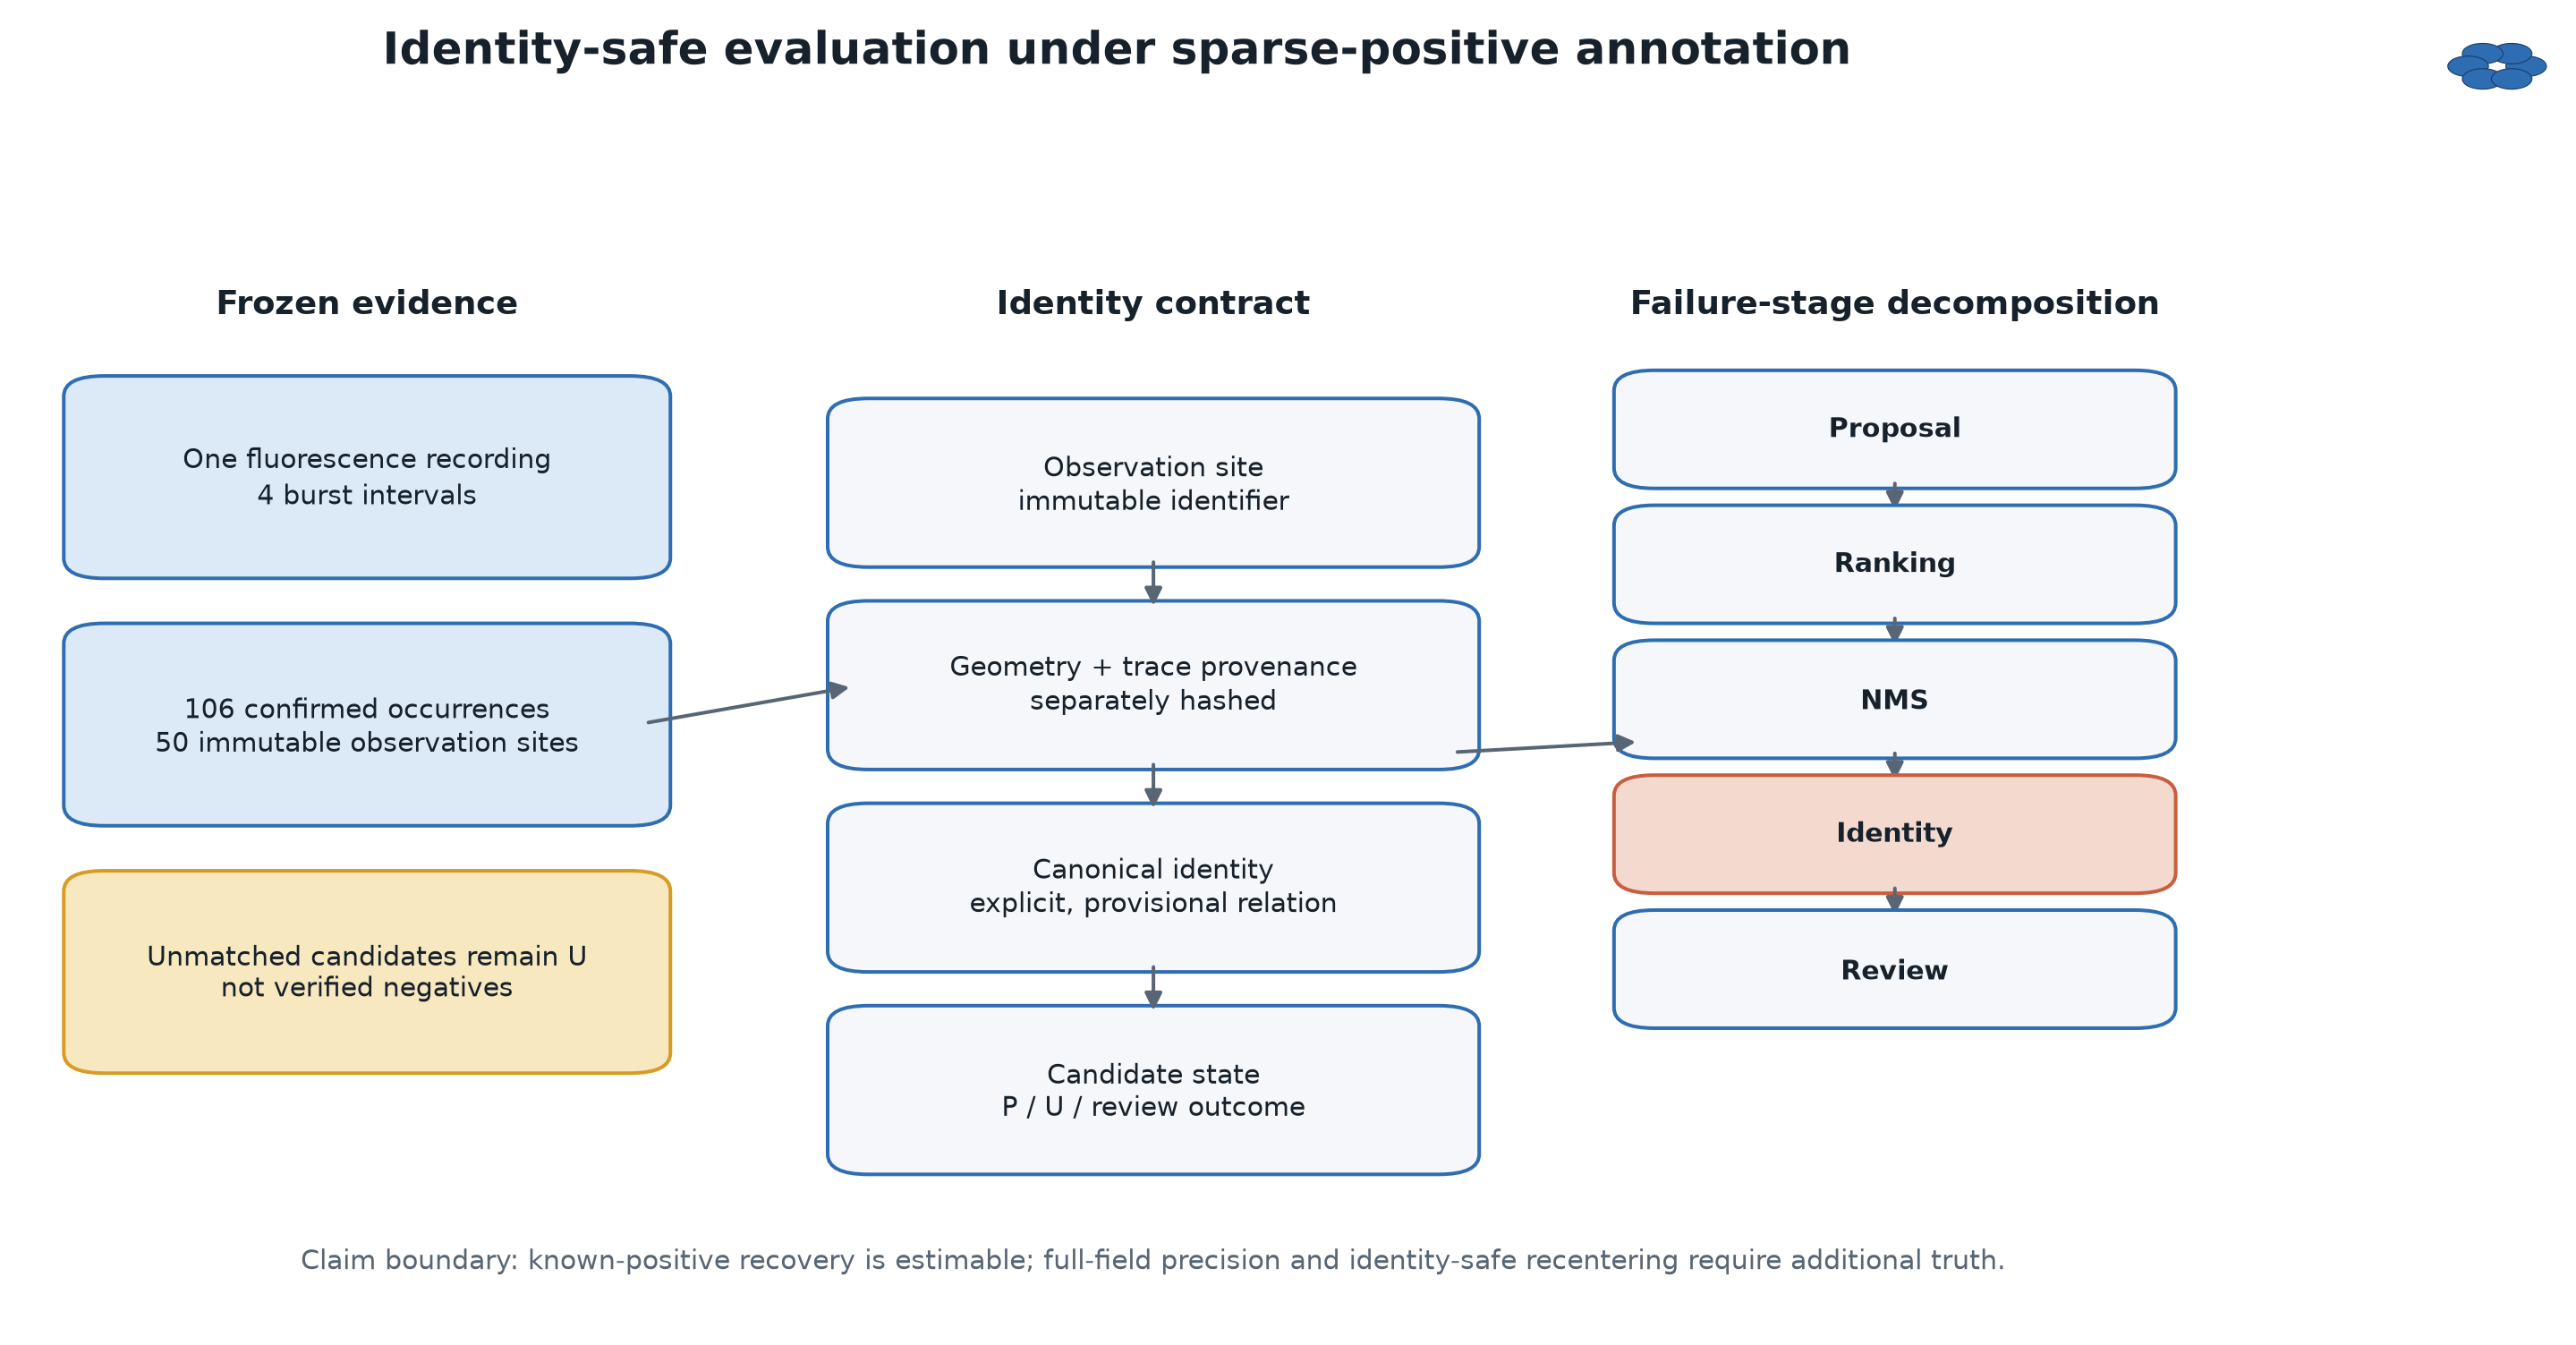
\includegraphics[width=\textwidth]{figures/venue/fig01_jnm_identity_contract.png}
  \caption{Identity-safe evaluation design. One recording and
  \VenueCohortBursts{} burst intervals yield \VenueCohortOccurrences{}
  confirmed occurrence-level geometries at \VenueCohortSites{} immutable
  observation sites. Spatial observations, geometry and trace provenance,
  provisional canonical identities, and unmatched candidates in state U are
  kept distinct. Proposal, ranking, non-maximum suppression, identity, and
  review are evaluated as separate failure stages.}
  \label{fig:venue-study-design}
\end{figure*}
